\chapter{Способ построения Актор-Критик САУ} \label{chapt2}

В подходе с обучением с подкреплением целью функционирования агента является максимизация целевой функции, который представляет собой суммарную величину награды - подкрепления. Такого типа управление относится к классу систем экстремального управления (СЭУ).

\section{Структурная схема системы экстремального управления} \label{sect2_1}
Системы экстремального управления относят к классу адаптивных систем, такие системы отличаются автоматическим выбором режима управления, при котором поддерживается минимальное или максимальное значение некой целевой функции. 

\begin{figure}[ht] 
  \center
  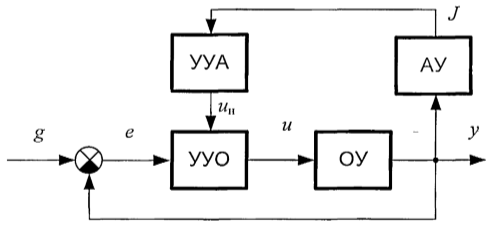
\includegraphics [scale=1] {seu_21}
  \caption{Структурная схема СЭУ} 
  \label{img:seu_21}  
\end{figure}



%\newpage
%============================================================================================================================
\section{Структурная схема Актор-Критик САУ} \label{sect2_2}
С помощью метода Актор-Критик и обучения с подкреплением разработана обобщенная структурная схема Актор-Критик САУ, изображенная на рисунке ~\ref{img:ac_struct}, а также алгоритмы функционирования системы
\begin{figure}[ht] 
	\center
	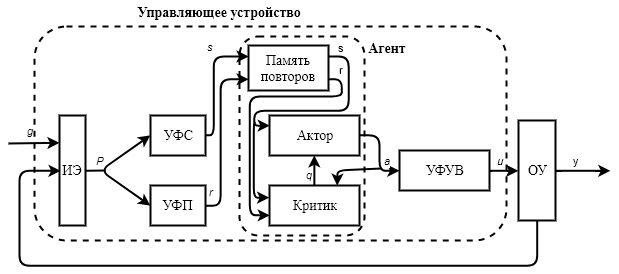
\includegraphics [scale=0.4] {ac_struct}
	\caption{Структурная схема Актор-Критик САУ} 
	\label{img:ac_struct}  
\end{figure}

\subsection{Импульсный элемент} \label{subsect2_2_1}
Целью функционирования импульсного элемента является дискретизация поступающего на вход сигнала с шагом $\tau$, который является параметром настройки УУ.

\subsection{Устройство формирования состояния} \label{subsect2_2_2}
Блок УФС отвечает за создание вектора состояний для Агента. 

\subsection{Устройство формирования подкрепления} \label{subsect2_2_3}

\subsection{Критик} \label{subsect2_2_4}

\subsection{Актор} \label{subsect2_2_5}

\subsection{Устройство формирования управляющего воздействия} \label{subsect2_2_6}

